\section{Sprint 9} % COMPARTICIÓN

\subsection{Planificación}

\textbf{Inicio: }?? del 2015 

\textbf{Fin:} ?? de octubre del 2015



\subsection{Descripción}

\subsection{User Stories relacionados}
La \textbf{Tabla \ref{US-Sprint9}} indicará las características de cada user story para guiarnos en el desarrollo del sprint.

\begin{table}[h]
    \label{US-Sprint9}
	%\resizebox{\textwidth}{!}{
    \centering
	\begin{tabular}{|l|p{9cm}|}
	\hline
        \multicolumn{1}{|c|}{\textbf{ID}} &
        \multicolumn{1}{|c|}{\textbf{Enunciado de la historia}} \\          
    \hline
        \textbf{US-2 } & Como paciente, quiero añadir al sistema los estudios realizados para evitar posibles perdidas.\\
     \hline 
     
    \end{tabular}
%     }

\end{table}

\subsection{Modelo de datos}
El Diagrama propio de este sprint se puede ver en la \textbf{Figura\ref{2-modelo_datos_general}}, allí se indican exactamente las clases que se usarán en este sprint y que serán detalladas con detenimiento en el presente documento. Se recuerda que se ha realizado un Diagrama de clases tentativo que se puede ver en la \textbf{Figura \ref{2-modelo_datos_general}}, dicho diagrama  será utilizado como base para este sprint y posee un alcance limitado el cual se irá modificando a medida que se profundice en los temas.





\subsection{Modelo funcional} %Diagrama de clases
Se describirán las funciones usando como marco de apoyo el sprint Backlog, además se armará el diagrama de casos de uso del presente Sprint \textbf{[Figura \ref{2-caso_de_uso2}]} que irá creciendo  medida se vaya avanzando en el proyecto.



    \begin{figure}[h]
        \centering
        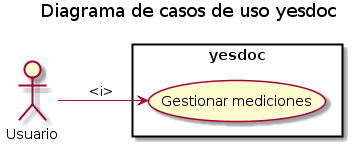
\includegraphics[width=0.5\textwidth]{img/2-caso_de_uso}
        \caption{formulario de edición de perfil}
		\label{2-caso_de_uso2}
    \end{figure}


\textbf{EJEMPLO}
	{\scriptsize
	\begin{center} %sidewaystable
	\centering
	%\begin{adjustbox}{max width=\textheight}
    \resizebox{\textwidth}{!}{
	\begin{tabular}{|l|l|l|l|}
	    \hline
	        \textbf{Area a cargo} &
	        \textbf{Responsable} &        
	        \textbf{Tarea} &
	        \textbf{US} \\
	    \hline
	    Front-end& Ivan Terreno & Generación de controladores para consumir Json de la Api relacionados a la API  & US-\ref{resumenInfo} \& US-\ref{infoSalud} \\ \hline

	    \end{tabular}
        }
	    %\end{adjustbox}
    	\end{center}
	}
    
    \textbf{Describimos cada tarea???}
\subsubsection{Creación de página de mediciones}

\subsection {Salidas del Sistema - Incrementos}
\textbf{Esto es un ejemplo. Debe listarse las pantallas y explicar que hacen}
\begin{enumerate}
    \item \textbf{Presentación de las últimas mediciones}  \textbf{[Figura  \ref{perfil_medicion}]} con posibilidad de edición de cada una de las mediciones. Los datos posible  a presentar son altura, peso, grasa corporal y glucosa. 
    
    La interfaz mostrará el valor de la medición, la fecha y hora en que fue realizada y la fuente que se utilizó para dicha medición.

\end{enumerate}

    




\subsection{Criterios de aceptación}
\textbf{Ejemplo - esto se debe modificar}
\begin{center}
\begin{longtable}{|p{0.5cm}|p{4cm}|p{4cm}|p{5cm}|}
\hline \hline \rowcolor[gray]{0.9}
	\multicolumn{4}{||c|}{\textbf{Criterio de aceptación}} \\
    \hline  \rowcolor[gray]{0.9}
        \textbf{Id} &
        \textbf{Contexto} &
        \textbf{Evento}&
        \textbf{Resultado} \\
    \hline
1&En caso de que exista una persona sin mediciones & cuando este desee observar sus mediciones  & El sistema no mostrará nada \\ \hline
 

  \end{longtable}
\end{center}


\subsection{Casos de prueba}

\subsubsection{Pruebas de integración entre módulos del Sistema}

\subsubsection{Pruebas de carga}

\subsubsection{Pruebas de seguridad por niveles de usuarios}


\subsection{Pruebas ejecutadas}
Aquí se realizará una conclusión general de lo que se descubrió en las pruebas.
        %
	\begin{itemize}
		\item \textbf{¿Que fue bien?}
        	\begin{itemize}
				\item        Las cargas y ediciones se llevan a cabo correctamente.
			\end{itemize}

   		\item \textbf{¿Que se mejoró?}
        	\begin{itemize}
                \item \textbf{Cerrado} problema
			\end{itemize}

   		\item \textbf{¿Que se puede mejorar?}
        	\begin{itemize}
		        \item \textbf{Abierto} En el futuro se deberá mejorar ...
            \end{itemize}
        

	\end{itemize}